\section{Introduction}

With the flourishing development of e-commerce platforms, online shopping has become a part of people's lives. To further stimulate online consumption, e-commerce platforms arrange various promotion campaigns on special days, such as Black Friday~\cite{2013Black} in Western countries and Double Eleven~\cite{double11} in China~\cite{huang2019x}. Along with numerous online promotions, some intermediate platforms have emerged in the market, such as Groupon~\cite{groupon} and Dealmoon~\cite{dealmoon}, which aim to help users sort out the hot promotions of various e-commerce platforms.

Unfortunately even some users know those promotions, they find it hard to meet the spending threshold to use a coupon or to enjoy the free delivery service. Therefore, users will intentionally seek for others, often their friends, to place the order together to meet the threshold. Because all the e-commerce platforms support only one shipping address for one order, when multiple users place an order together, one of the users will inevitably receive all the products first and then distribute them to others respectively. These complex processes are unreliable and time-consuming for consumers. What is even more damaging to consumers' motivation to shopping is that increasingly complicated e-commerce promotion activities impose extra workloads to customers, since multiple complex coupons rules may change on a daily basis~\cite{double2020}.
\begin{figure}[t]\vspace{-2ex} 
\centering %图片居中
		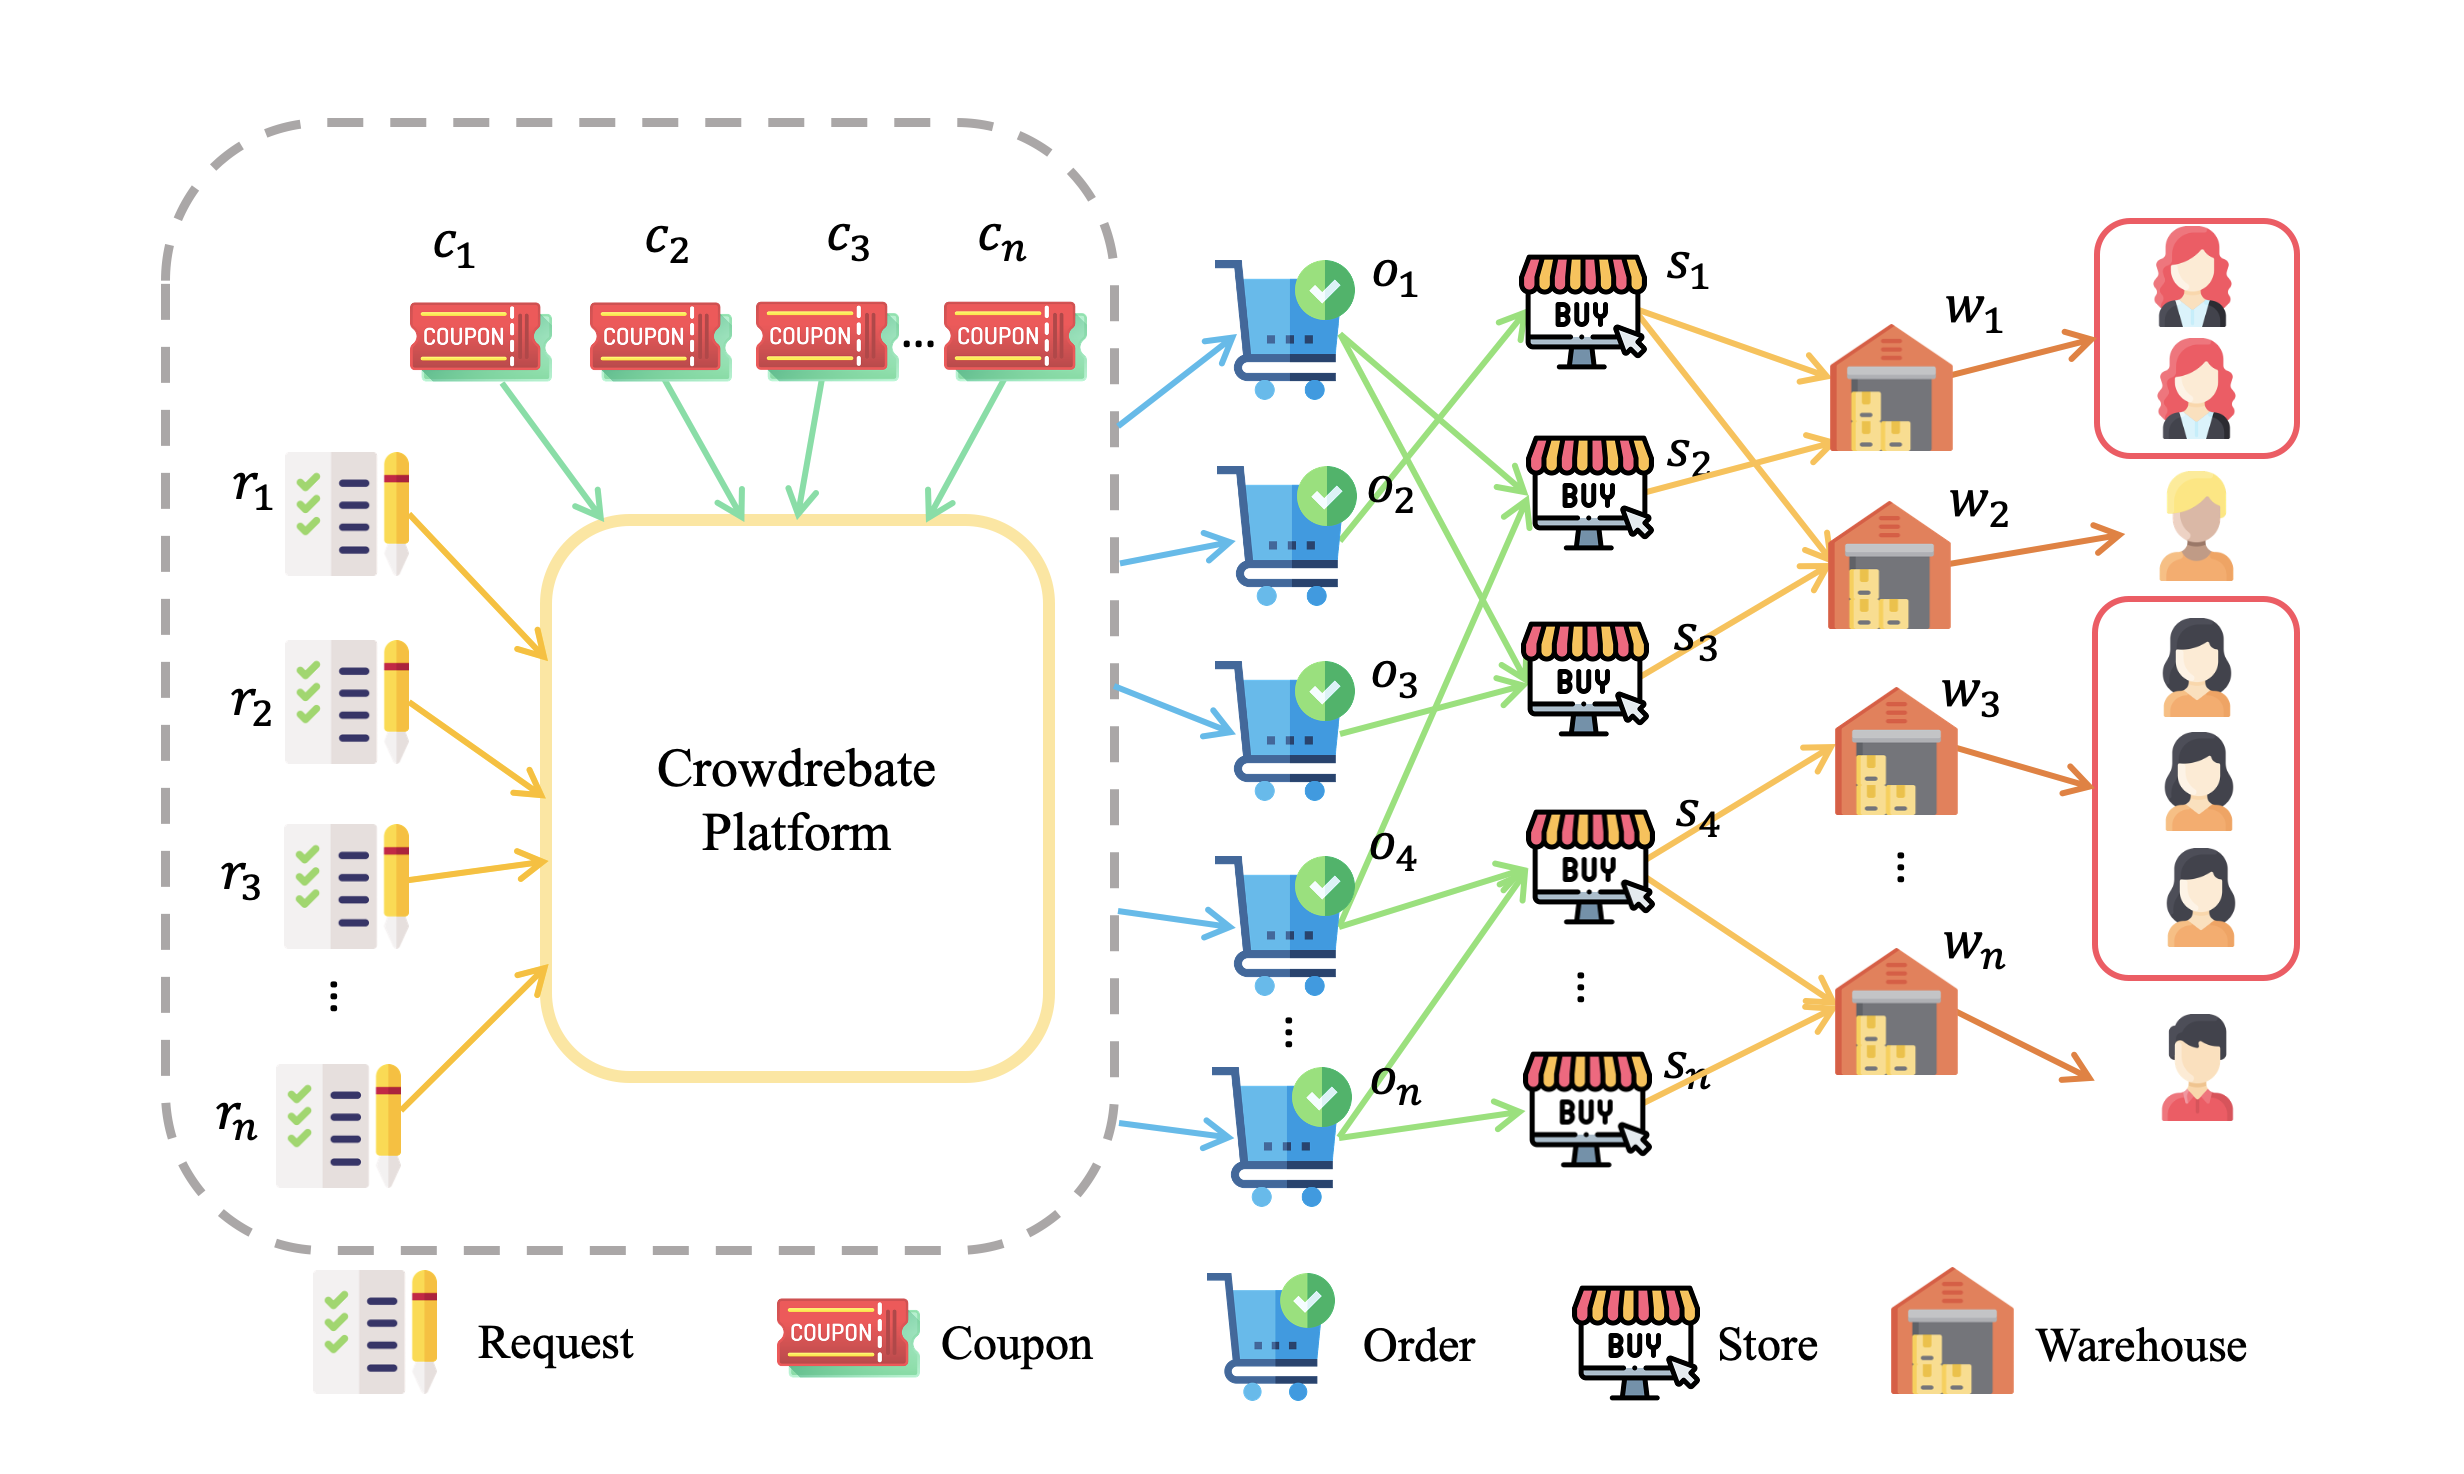
\includegraphics[width=0.5\textwidth]{../figure/crowdrebate process.png} %插入图片,[]中设置图片大小,{}中是图片文件名
	\caption{The operation process of Crowdrebate} %最终文档中希望显示的图片标题
	\label{fig:Crowdrebate} %用于文内引用的标签
	\vspace{-3ex}
	\end{figure}

Under these circumstances, our demo-Crowdrebate firmly addresses consumers' pain points. Crowdrebate collects users' purchasing requests and group their requests even users do not know each other into orders to maximize total benefit. Meanwhile, we give the exposure of online retailers' promotions so that more users would participate in promotions. To summarize, not only do we dedicate ourselves to help users get more benefits, we also devote ourselves to help e-commerce platforms fill more orders, increase platforms’ revenue, and ultimately achieve a bilateral win-win situation.

Our platform operates as follows as shown in Figure~\ref{fig:Crowdrebate}. Users can post their requirements corresponding to the information of the desired product. Based on the received requests, we make an order grouping and match the suitable coupons, using our \emph{crowdrebate algorithm}~\cite{Report}, to maximize each order's rebate deducting the delivery costs. Because we place the orders for consumers, the products are first sent to our warehouses from the online stores, and then we will distribute the products according to the users. The site of our warehouses considers the distribution of the user load as evenly as possible. The specific system architecture we will introduce in the next section.

Generally, Crowdrebate consists of three components. The user interface provides service for users to post requests and track data. The algorithm function supports our core features, group ordering and recommendation. The data manager handles business logic and data storage.

Thus, our demo has following contributions:
\begin{itemize}
	\item We develop a platform for users to post for group ordering and track realtime information on mobile phones.
	\item We design two algorithms to combine orders for maximum rebates under different scenarios.
	\item We equip the platform with process automation and recommendation to handle large scale data and enrich users experience.
\end{itemize}
\begin{figure}[t] \vspace{-2ex}
	\centering %图片居中
	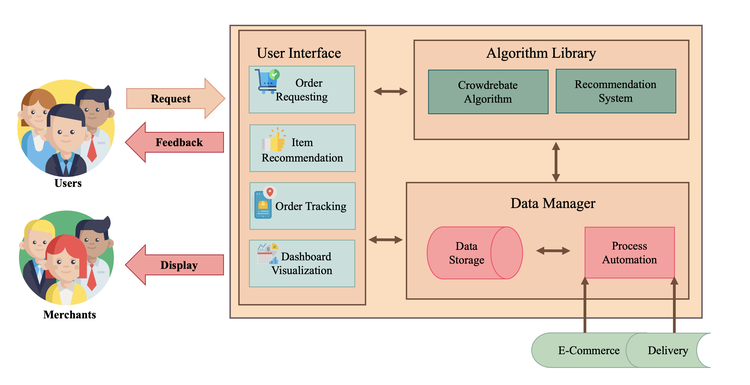
\includegraphics[width=0.5\textwidth]{../figure/ar.png} %插入图片,[]中设置图片大小,{}中是图片文件名
	\caption{The architecture of crowdrebate} %最终文档中希望显示的图片标题
	\label{fig:ar} %用于文内引用的标签
	\vspace{-3ex}
\end{figure}

